\begin{figure}[p]
    \centering
    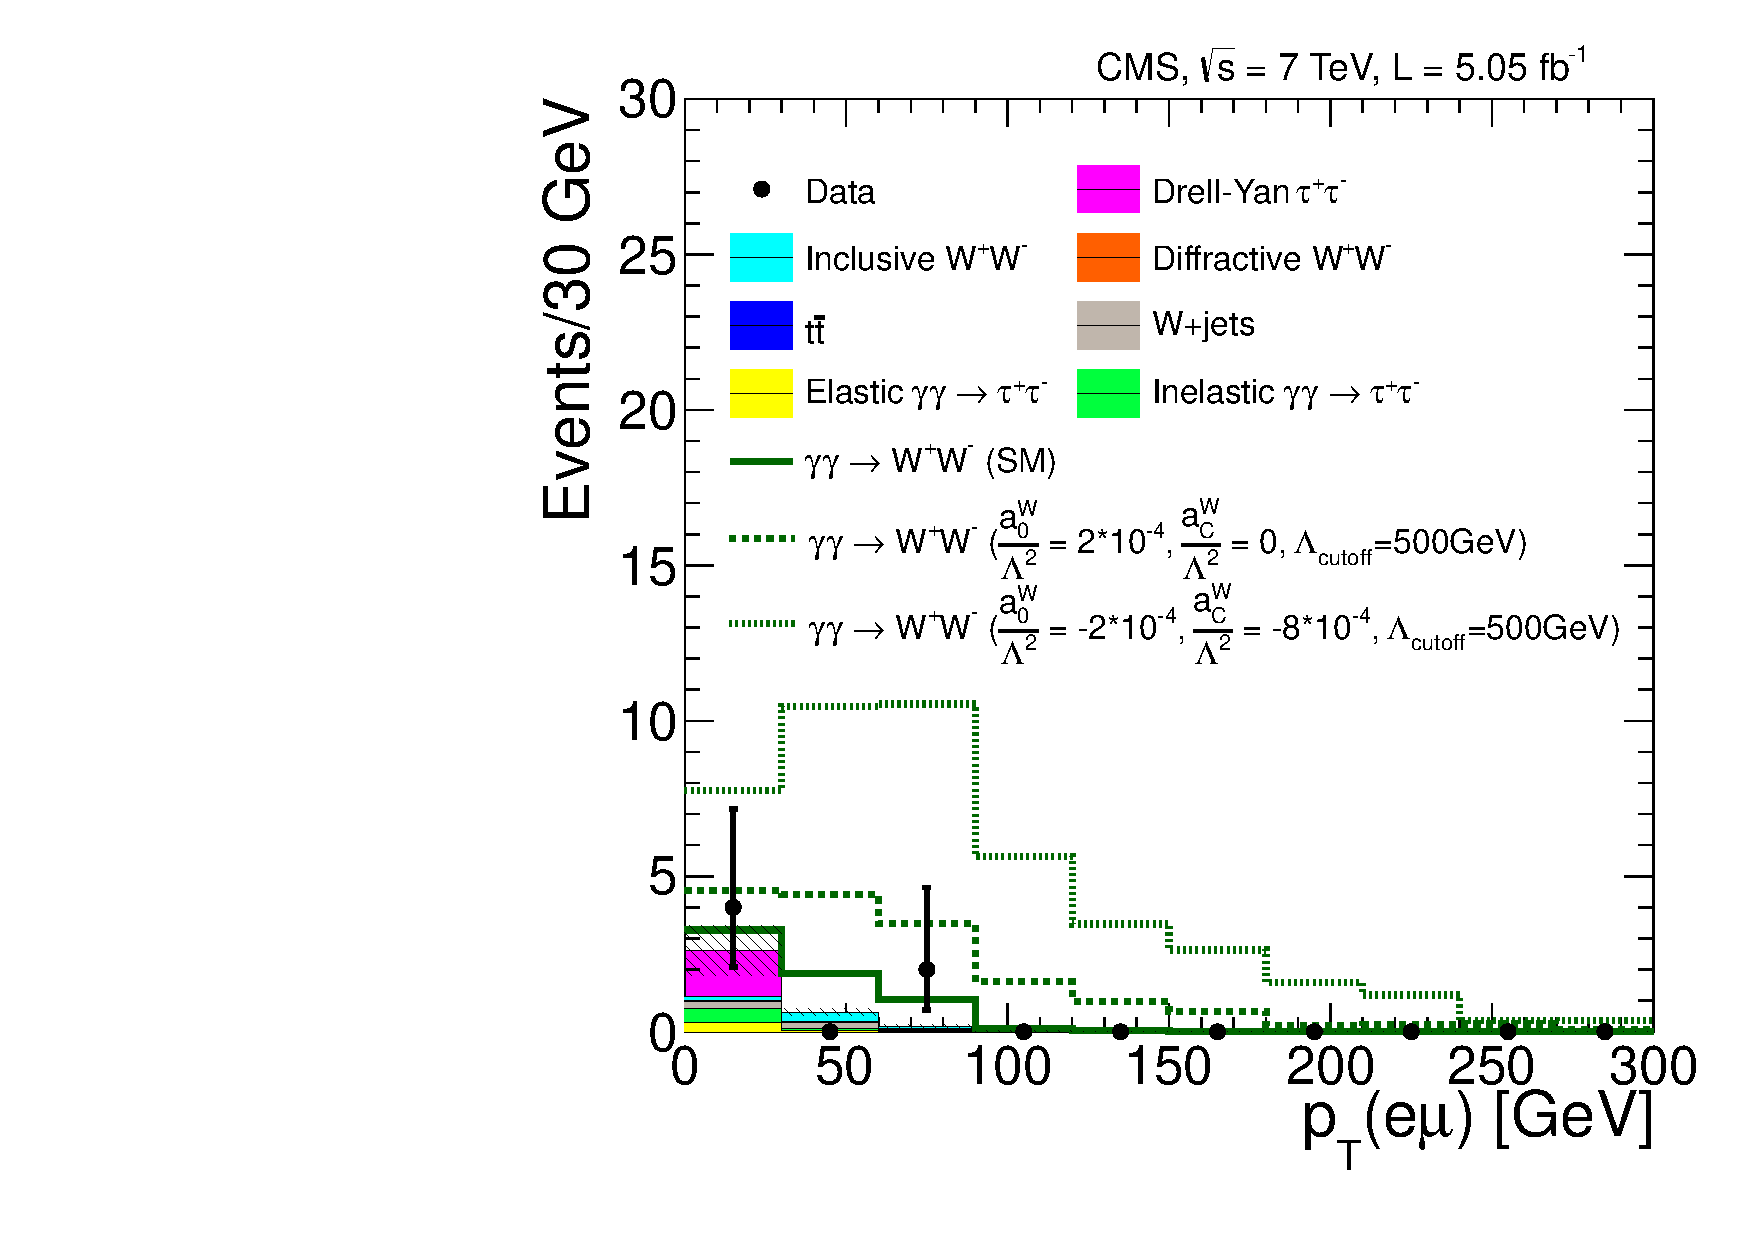
\includegraphics[height=0.3\textheight]{figures/ss-exclboson-ww-cms7tev}
    \caption{}
    \label{fig:ss-exclboson-ww-cms7tev}
\end{figure}
CMS WWexcl 7 \TeV~\cite{Chatrchyan:2013foa}
ATLAS SSWW 8 \TeV~\cite{Aad:2014zda}
CMS SSWW 8 \TeV~\cite{Khachatryan:2014sta}


\begin{figure*}[htb] {
\centering
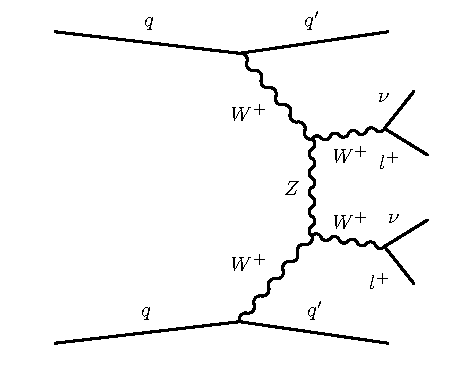
\includegraphics[width=0.315\textwidth]{figures/ss-exclboson-ww-diagram1.pdf}
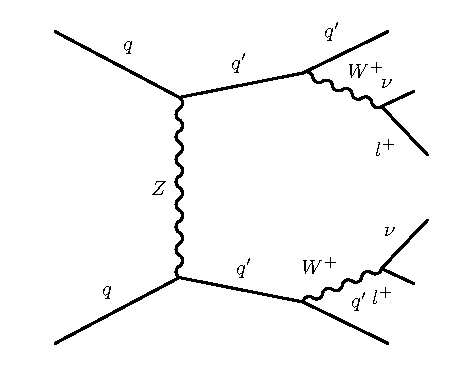
\includegraphics[width=0.35\textwidth]{figures/ss-exclboson-ww-diagram2.pdf}
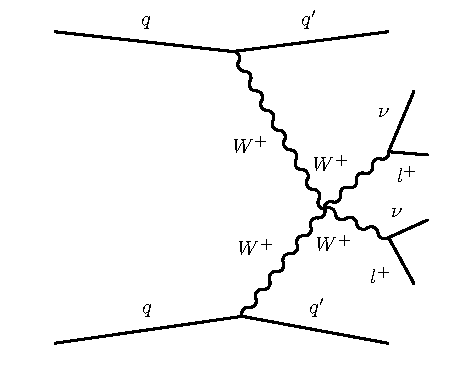
\includegraphics[width=0.315\textwidth]{figures/ss-exclboson-ww-diagram3.pdf}
\caption{
Representative Feynman diagrams for same-sign $WW$ production in association
with two jets from purely electroweak contributions:
(left) vector boson fusion,
(middle) bremsstrahlung-like,
and (right) multiperipheral production.
\label{fig:ss-exclboson-ww-sigdiagram}}

}
\end{figure*}


\begin{figure}[p]
    \centering
    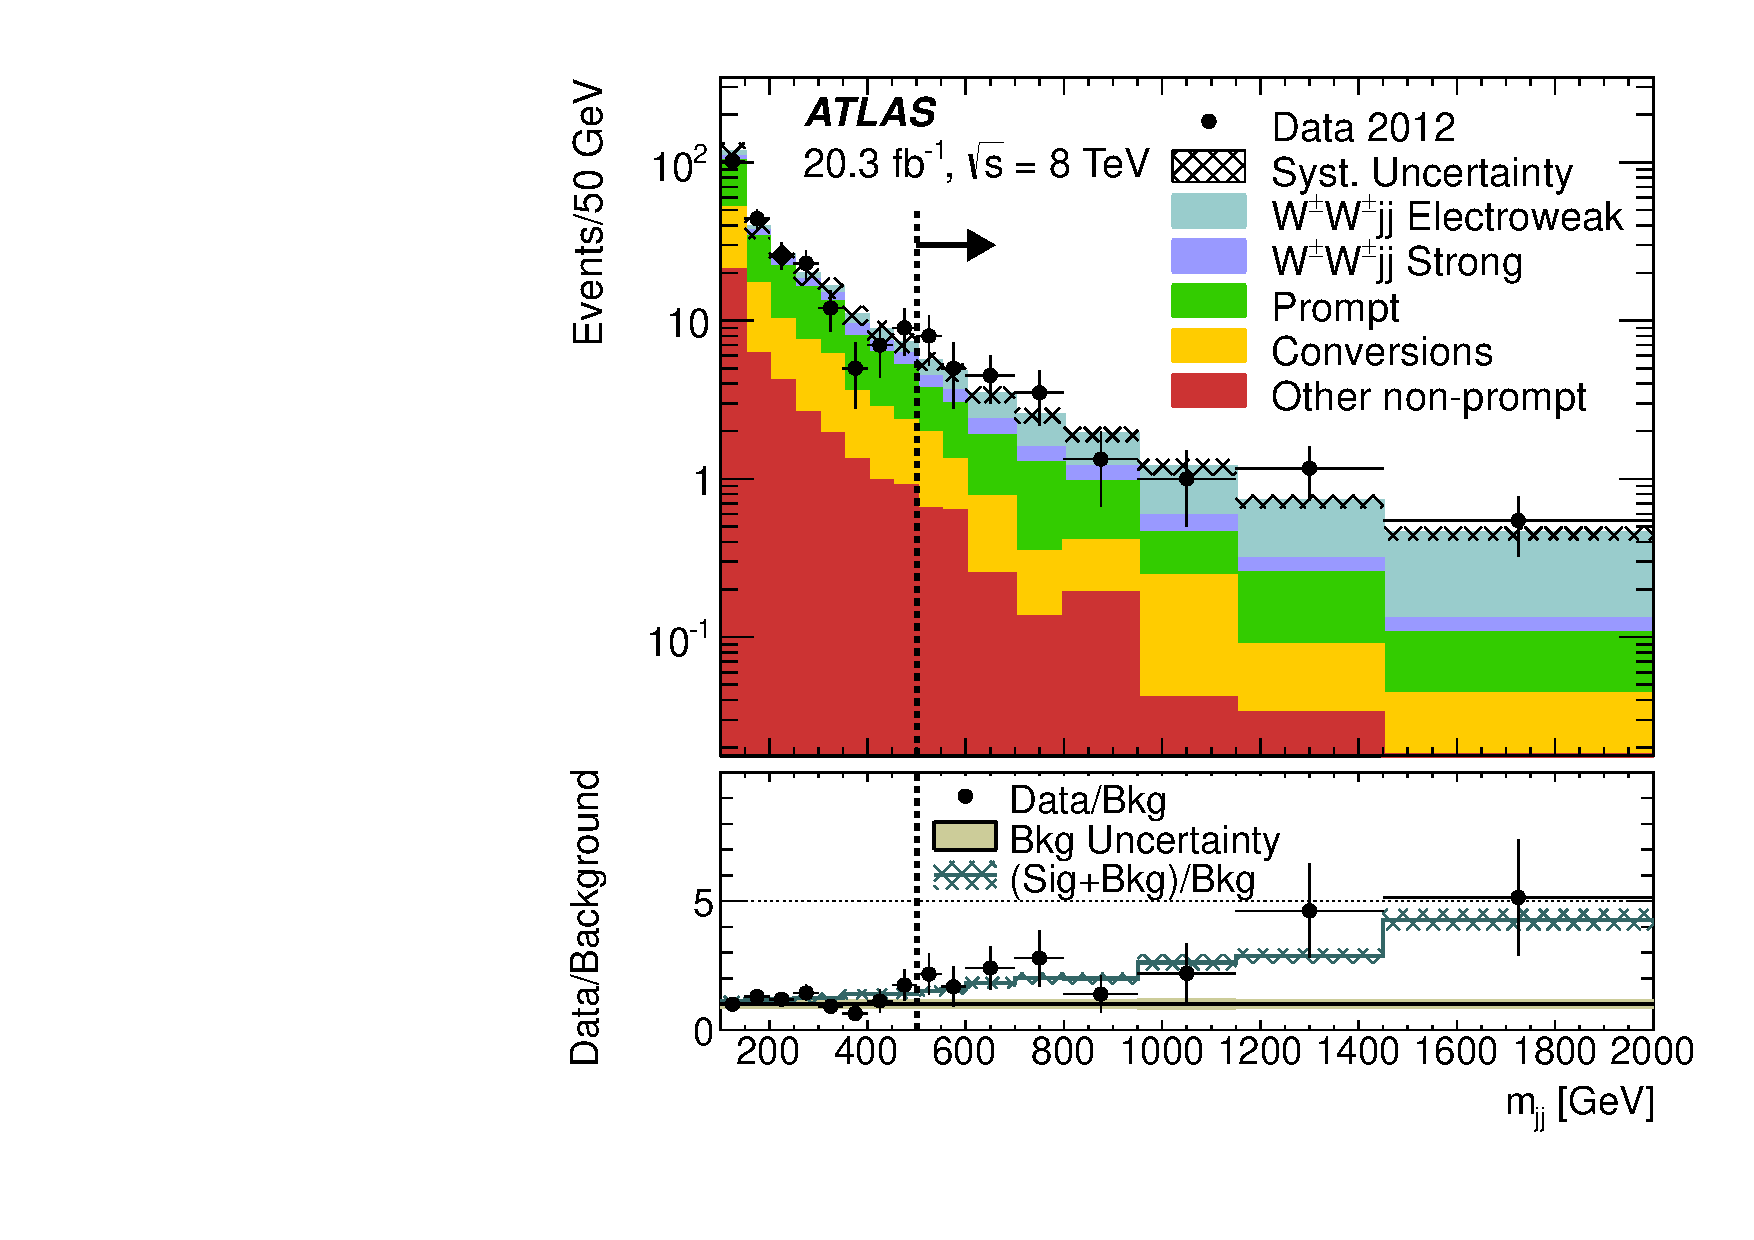
\includegraphics[width=0.45\textwidth]{figures/ss-exclboson-ww-ss-atlas8tev.pdf}
    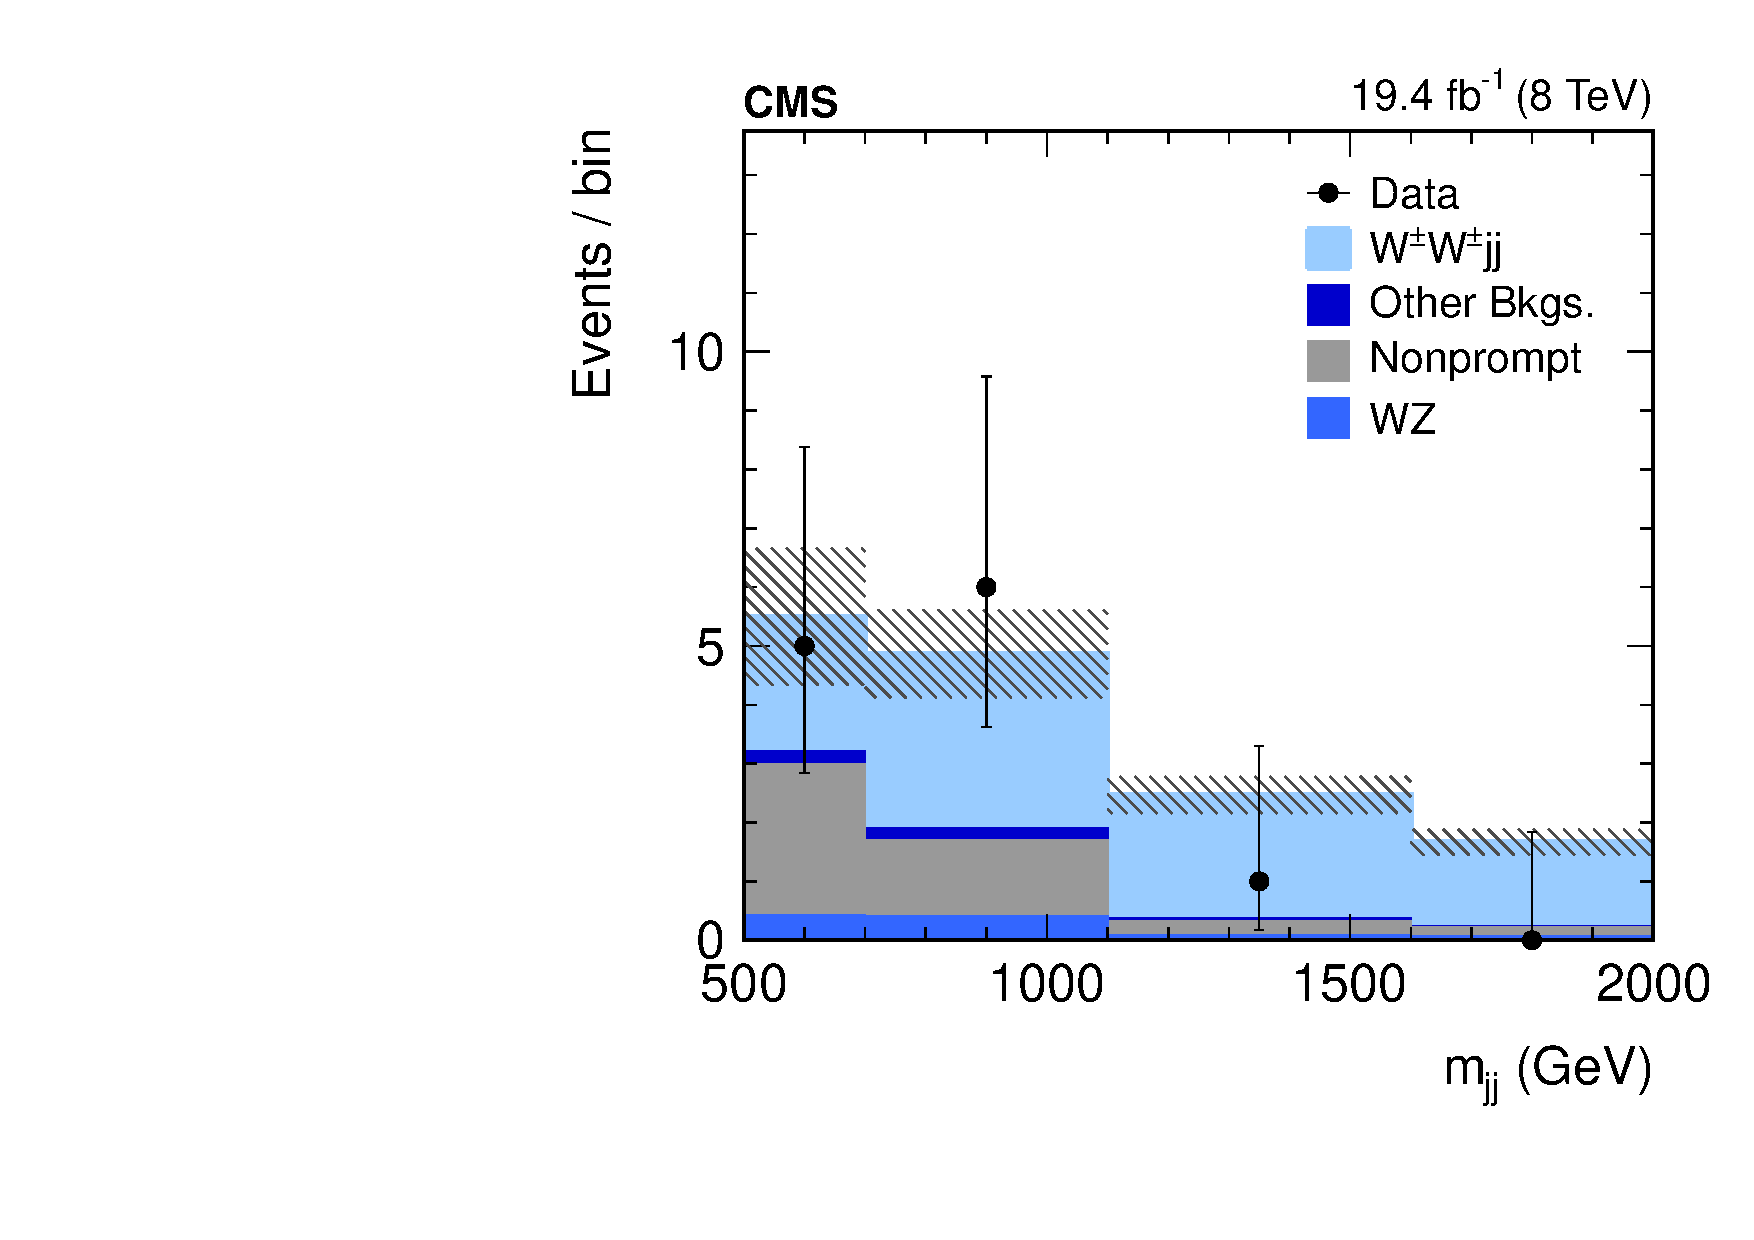
\includegraphics[width=0.45\textwidth]{figures/ss-exclboson-ww-ss-cms8tev.pdf}
    \caption{
    Left:  a signal region by ATLAS.
    Right:  }
    \label{fig:ss-exclboson-ww-ss}
\end{figure}
